\documentclass{article}
\usepackage[utf8]{inputenc}
\usepackage{natbib}
\usepackage{graphicx}
\usepackage[space]{grffile}
\usepackage{lastpage}
\usepackage{xcolor}
\usepackage{lipsum}
\usepackage[T1]{fontenc}
\usepackage{fancyhdr}
\usepackage{geometry}
\usepackage{url}
\usepackage[dutch]{babel}
\usepackage[bottom]{footmisc}
\usepackage[toc,page]{appendix}
\usepackage{footnote}


\bibliographystyle{abbrv} %abbrvnat geeft problemen

\title{Software Design Document}
\author{} %leave empty
\date{14 mei 2015} %ok, manuele datum

\addtolength{\footskip}{1.3cm} % make more space for the footer
\pagestyle{fancyplain} % use fancy for all pages except chapter start
\lhead{}
\cfoot{
\includegraphics[height=1.3cm]{Small_Logo.png}} % right logo
\rfoot{\thepage}
\renewcommand{\headrulewidth}{0.3pt} % remove rule below header
\renewcommand{\footrulewidth}{0.3pt} % remove rule below header
\newcommand{\myparagraph}[1]{\paragraph{#1}\mbox{}\\}

\begin{document}

\makeatletter
\begin{titlepage}

\newcommand{\HRule}{\rule{\linewidth}{0.7mm}} % Defines a new command for the horizontal lines, change thickness here


\vspace*{1.2mm}

\center 

\includegraphics[scale=0.6]{Logo.png}\\[1cm] 
%---------------------------------------------------------------------------------------
%	HEADINGS SECTION
%----------------------------------------------------------------------------------------

\textsc{\LARGE Vrije Universiteit Brussel}\\[0.3cm] % Name of your university/college
\textsc{\large WE-DINF-6537}\\
\textsc{\large Project Software Engineering}\\
\textsc{\large Academiejaar 2014-2015}\\[0.3cm] 
%\textsc{\large Software Engineering}\\[0.7cm] % Major heading such as course name

%----------------------------------------------------------------------------------------
%	TITLE SECTION
%----------------------------------------------------------------------------------------

\HRule \\[0.4cm]
{ \huge \bfseries \@title \\[0.5cm] }
\HRule \\[0.5cm]
 
%----------------------------------------------------------------------------------------
%	AUTHOR SECTION
%----------------------------------------------------------------------------------------

\Large
% laat voorlopig nog even de namen/mailadressen op deze pagina staan
% eerst moeten we zien of er een beter alternatief is om de lege plek dan op te vullen
% anders laten we ze gewoon staan...

%volgens mij ziet het er zo heel goed uit, maar als ze echt wegmoeten mss vub logo groter maken? 
% => OK, ik vind het ook veter zo, we laten ze staan!
Douglas Horemans \textit{<dhoreman@vub.ac.be>}\\
Hannah Pinson \textit{<hpinson@vub.ac.be>}\\
Ivo Vervlimmeren \textit{<ivervlim@vub.ac.be>}\\
Noah Van Es \textit{<noahves@vub.ac.be>}\\
Pieter Steyaert \textit{<psteyaer@vub.ac.be>}\\

\vspace{0.6cm}


\includegraphics[scale=0.4]{VUB_schild.pdf}\\[0.5cm]

{\large 19 november 2014}
\vfill % Fill the rest of the page with whitespace

\end{titlepage}

\newpage
\section*{Versiegeschiedenis}
\addcontentsline{toc}{section}{Versiegeschiedenis}

\begin{center}
\begin{tabular}[t]{| c | c | c | c |}
    \hline
    \textbf{Versie} & \textbf{Datum} & \textbf{Auteurs\cite{note:author}} & \textbf{Beschrijving} \\
    \hline
    
    1.0     &  19/11/2014   &   \begin{tabular}{c} 
                                    Douglas Horemans \\
                                \end{tabular} & Eerste versie \\
    \hline
    2.0     &  15/12/2014   &   \begin{tabular}{c} 
                                    Douglas Horemans \\
                                \end{tabular} & tweede versie \\
    \hline
\end{tabular}
\end{center}
\newpage



\tableofcontents
\newpage

\section{Introductie}

\subsection{Doel}

Dit document beschrijft de architectuur van de software achter SKRIBL. 
Het analyseert het ontwerp en haar (sub)compomenten en geeft een beschrijving
van de werking van het systeem. Op die manier geeft het dus de nodige richtlijnen
voor de implementatie en wordt de filosofie achter het design toegelicht.
Daarnaast geeft het ook aan hoe gebruikers het systeem kunnen gebruiken, zowel
via de grafische webinterface als via een aparte API voor third-parties.

\subsection{Scope}

SKRIBL is een webapplicatie die gebruikers toelaat om publicaties met elkaar te delen
en te beheren op een interactieve manier. De bedoeling is dus dat men zowel eigen publicaties kan uploaden, alsook op zoek kan gaan naar andere publicaties en zo dus een volledig netwerk kan opbouwen binnen zijn/haar onderzoeksdomein. Het systeem moet hiervoor ook de nodige interface en visualisaties aanbieden, zowel in normale desktop-browsers als voor mobiele apparaten.

Hiervoor zal de software worden uitgerust met een databank en de nodige applicatielogica om aan alle software eisen te voldoen. Ook moet het systeem rekening houden met de webarchitectuur en bekijken hoe de modules en verantwoordelijkheden worden verdeeld onder de client en de server. Voor een volledig overzicht van de beoogde functionaliteit wordt verwezen naar het SRS ~\cite{Xtreport:SRS}.

\subsection{Overzicht}

Eerst en vooral wordt er in dit document gekeken naar de globale structuur van de software. Hierbij wordt het systeem eerst in grote lijnen besproken, waarna elk onderdeel vervolgens meer in detail wordt bekeken. Daarnaast wordt ook kort de filosofie van het ontwerp toegelicht. 
Vervolgens wordt er gekeken naar de organisatie van de informatie binnen het systeem. Hierbij worden onder andere een schema van de database en diagrammen meegegeven om aan te geven welke data hoe wordt opgeslagen en gebruikt. 
Daarna wordt op een systematische manier bekeken wat elk component binnen het systeem doet. Concreet wordt hier bijvoorbeeld aangegeven hoe een bepaalde methode of algoritme precies werkt.

Nadien volgt een beschrijving van de interfaces, zowel van de grafische webomgeving als van de API. In dit gedeelte kan men terugvinden hoe het systeem gebruikt kan worden en wordt het verloop van de mogelijke handelingen beschreven. Deze handelingen zijn voornamelijk gebaseerd op de requirements zoals opgesteld in het SRS~\cite{Xtreport:SRS}. \\

De opmaak van dit document is gebaseerd op de IEEE 1016-1998 standaard voor SDD's~\citep{website:IEEE}.

\subsection{Referentiemateriaal}
\begingroup
\renewcommand{\section}[2]{}  % verwijdert titel sectie referenties
\bibliography{referenties}
\endgroup
 
\subsection{Definities en Acroniemen}

\begin{description}

\item[SRS] Software Requirements Specification
\item[SPMP] Software Project Management Plan
\item[SDD] Software Design Document
\item[MVC] Model-View-Controller
\item[API] Application Programming Interface
\item[GUI] Graphical User Interface
\item[SPA] Single-Page Application
\item[JSON] JavaScript Object Notation
\item[AJAX] Asynchronous Javascript and XML
\item[DMBS] Database Management System
\item[(E)ER] (Extended) Entity-Relation
\item[SQL] Structured Query Language
\item[REST] Representational State Transfer
\item[HTML] Hypertext Markup Language
\item[HTTP] Hypertext Transfer Protocol
\item[URL] Uniform Resource Locator
\item[DOM] Document Object Model
\item[SSL] Secure Sockets Layer
\item[CSS] Cascading Style Sheets
\item[JS] Javascript

\end{description}

\clearpage

\section{Systeemoverzicht}

\subsection{Context}

De software wordt opgeleverd in de de vorm van een webapplicatie. Dit houdt in dat op de server een HTTP(S)-server zal draaien en de client vanuit de browser hiernaar requests zal sturen via een webinterface, ontworpen voor zowel mobiele als desktop-clients.

\subsection{Organisatie}

De software zal worden ontwikkeld volgens de principes van het Agile Development Proces. Zo zal de implementatie van de componenten die in dit document worden beschreven verlopen in verschillende iteraties en sprints. Voor een gedetailleerde beschrijving en planning van deze sprints wordt verwezen naar het SPMP ~\cite{Xtreport:SPMP}.

\subsection{Gebruikte technologie\"en}

Om het systeem te ontwikkelen wordt gebruik gemaakt van een zuivere \textbf{`HTML/CSS/JS'}-stack.
Daarnaast zullen ook volgende open-source frameworks en libraries worden gebruikt:

\begin{itemize}

\item \textbf{ExpressJS} zal worden gebruikt als framework om de webapplicatie te ontwikkelen en zo gemakkelijker een API voor de server te kunnen ontwerpen\cite{website:ExpressJS}. 

\item \textbf{OrientDB} zal dan weer gebruikt worden als DMBS~\cite{website:OrientDB}. OrientDB is een zogeheten NoSQL-database, waarbij data niet wordt georganiseerd in tabellen zoals in een conventionele SQL-database. Specifiek zal gebruik worden gemaakt van de GraphDB-abstractie die OrientDB aanbiedt bovenop hun standaard database. 
Dit laat toe om om alle informatie rondom gebruikers, publicaties, ... in SKRIBL te modelleren als een graaf. Voor de communicatie over het binary protocol wordt gebruik gemaakt van oriento.~\cite{website:Oriento}

\item \textbf{AJAX} zal op de client worden gebruikt om op een asynchrone (en dus gebruiksvriendelijke) manier requests te sturen naar de server en vervolgens de UI te updaten. Deze technologie is van cruciaal belang om te voldoen aan de design filosofie die wordt beschreven in \ref{sec:rationale}.

\item Daarnaast zal voor de front-end gebruik worden gemaakt van \textbf{AngularJS}. AngularJS  is een zeer flexibel MVC-framework dat HTML uitbreidt met specifieke directives, controllers, \dots~\cite{website:AngularJS}. 

\item \textbf{Cheerio}~\cite{website:cheerio} wordt gebruikt om aan \textit{web scraping} te doen. Het implementeert een subset van jQuery zodat de HTML-pagina van een website kan worden gemanipuleerd aan het hand van het DOM-object. Zo kan bijvoorbeeld informatie worden gezocht op een website indien er geen API beschikbaar is.


\end{itemize}


Ten slotte zal de server als onderliggende (open-source) runtime gebruik maken van \textbf{NodeJS}. NodeJS maakt het mogelijk om ook server-side Javascript te gebruiken met een performant event-driven (m.a.w. asynchroon, non-blocking) model~\cite{website:NodeJS}. 
\clearpage

\section{Systeemarchitectuur}

\subsection{Design Rationale}
\label{sec:rationale}

Deze sectie bespreekt eerst de algemene filosofie en structuur achter het ontwerp. Veel van deze principes zijn gebaseerd op het concept van `Web 2.0'-applicaties.
Er is gekozen om gebruik te maken van een MVC-structuur om de applicatielogica (`model') en de UI (`view') gescheiden te houden. 
Hieronder vindt men een grafische voorstelling van dit concept:

\begin{figure}[!h]
\centering
 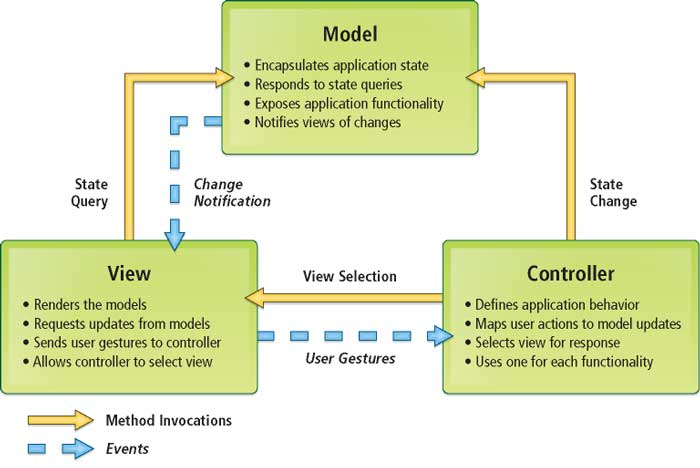
\includegraphics[width=130mm]{MVC.jpg}
 \caption{Illustratie van het MVC-patroon}
 \label{Model-View-Controller}
\end{figure}

\thispagestyle{fancy}
Hierbij zal de webserver voornamelijk de rol van M op zich nemen, terwijl de client de VC-rollen zelf zal beheren. We kunnen hier dus niet langer spreken over een thin, maar wel over een Rich client \footnote{Rich betekent hier niet noodzakelijk `fat'; onder model wordt ook de applicatielogica rondom dit model verstaan, waardoor de server nog altijd deze belangrijke functies zal moeten implementeren.}. 

De applicatie wordt hierdoor een Single-Page Application (SPA), waarbij alle functionaliteit van de server wordt vrijgegeven via een RESTFul API. Hierdoor wordt het gemakkelijker om later aparte desktop en mobiele versies aan te maken en kunnen ook andere developers gebruik maken van SKRIBL.

\subsection{Architectuur}

De architectuur kan men dan indelen in een three-tier model met een client tier, server tier, en database tier. Op de client tier gebeurt alle user-interactie met de view en wordt de front-end applicatie beheerd via controllers. Deze zullen de nodige gegevens halen via de (RESTful) API van de server, die ook de voornaamste services aan de front-end zal leveren. \\ 
Voor de uiteindelijke interactie met de data zelf, zal deze server-tier ook communiceren met de database-tier, waarop de OrientDB-database zich bevindt. \\
Hieronder vindt men een visualisatie van deze architectuur:

\begin{figure}[!h]
\centering
 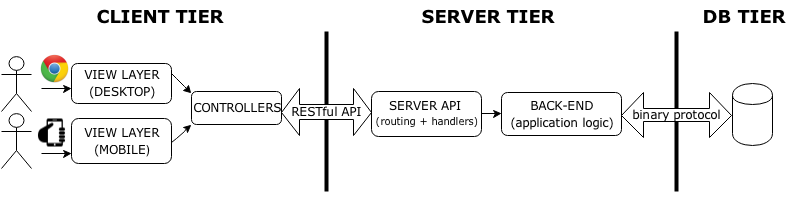
\includegraphics[width=140mm]{Architecture.png}
 \caption{Verschillende tiers in de webapplicatie}
 \label{Architecture}
\end{figure}

\subsection{Decompositie}

Hier word een beknopt overzicht gegeven van de verschillende onderdelen uit bovenstaande architectuur. Voor een gedetailleerde beschrijving van hun individuele componenten wordt verwezen naar sectie~\ref{sec:components}.

\subsubsection{Client Tier}

\paragraph{Views} 
De views vormen op de client-tier de GUI voor de eindgebruiker en verschillen voor desktop en mobiele gebruikers. Om het concept van de Single-Page Application te verwezenlijken, zal de server daarom bij bezoek van de website een template aanleveren, afhankelijk van het apparaattype van de gebruiker. Deze template zal gebruik maken van AngularJS en voldoende applicatielogica bevatten (geconfigureerd via de controllers) om tijdens het verloop van de applicatie zelf de interface te laten evolueren. De opmaak en structuur ervan gebeuren aan de hand van HTML \& CSS.

Er zullen, vanwege de verschillende weergave- en invoermogelijkheden van de apparaten, aparte views nodig zijn om zowel mobiele als desktop-gebruikers te ondersteunen. Hierbij is het wel de bedoeling dat zoveel mogelijk code uit de controllers kan worden hergebruikt, wat mogelijk is dankzij de scheiding tussen view en controller die wordt aangeboden door het MVC-patroon.

\paragraph{Controllers} 
De controllers zullen via de AngularJS-directive `ng-controller' worden verbonden aan de views en handelingen van de gebruiker verwerken. Meestal houdt dit in dat een AJAX-call naar de server zal worden gemaakt en het resultaat (meestal in JSON-formaat) geparsed en gebruikt zal worden om zo de view te updaten.

De controllers dragen daarnaast ook de verantwoordelijkheid om de 'flow' van de applicatie te beheren. De server is (volgens de REST-principes) stateless en houdt dus geen sessiegegevens bij. Het is dus de taak van de controllers om bijvoorbeeld bij te houden welke gebruiker is ingelogd en waar hij/zij mee bezig is. In feite biedt de Server Tier enkel een interface aan voor de gegevens die in de applicatie moeten worden weergegeven.

\subsubsection{Server Tier}

\paragraph{Server API} 
Dit gedeelte van de Server API is verantwoordelijk voor het afhandelen van requests van de client. Afhankelijk van het type request en de route (path) zal een bepaalde handler worden opgeroepen die gebruik zal maken van de back-end om de bijhorende applicatielogica uit te voeren en het juiste resultaat naar de client terug te sturen. Als ingangspunt van de server-tier is dit gedeelte dus ook verantwoordelijk voor het opstellen van de RESTful API.

\paragraph{Back-end} 
De back-end voorziet in de meeste functionaliteit van de applicatie. Hoewel de applicatie er voornamelijk in bestaat gegevens in het model correct op te slaan (via de database-tier), is er ook een aparte laag nodig voor de applicatielogica. Deze bevindt zich voor het grootste deel op de server en wordt op de back-end in aparte modules afgehandeld.

Hierbij gaat het vooral over de verwerking van de gegevens zoals gebruikers en publicaties. De back-end zal bijvoorbeeld zorgen voor de server-side validatie van gebruikersinput en zal ook de extractie van gegevens (metadata) uit publicaties op zich nemen. Ook complexere operaties op de database, die nodig zijn om bepaalde features te implementeren, zullen hier terug te vinden zijn.

\subsubsection{Database Tier}

Ten slotte zal op de database-tier een server worden opgezet met een database door OrientDB. Het volstaat hier om gewoon via de command-line een meegeleverd shell-script uit te voeren om deze server op te starten.
Een gedetailleerde beschrijving van het ontwerp van deze database volgt in de volgende sectie. 

\clearpage

\section{Data design}
\label{sec:data}

De organisatie van data is cruciaal bij het ontwerp van SKRIBL. Een effici\"ente en persistente datastructuur is nodig om alle relaties tussen de verschillende entiteiten (gebruikers, publicaties, onderzoeksdomeinen, ...) in de applicatie te kunnen modelleren. \\

Om die reden werd gekozen om gebruik te maken van een graph-database. Een graf is veruit de meest natuurlijke representatie van het model en maakte het later ook gemakkelijker om verbanden in de applicatie te verwerken en te visualiseren. 

Concreet werd er gekozen voor OrientDB omdat deze bovenop haar NoSQL-database ook een abstractie aanbiedt die specifiek is ontworpen om graph-databases in elkaar te steken. Daarnaast is het ook een performante DBMS met een gebruiksvriendelijke API. \\

Wat volgt is een (E)ER-model van de huidige structuur in de database.

\begin{figure}[!h]
\centering
 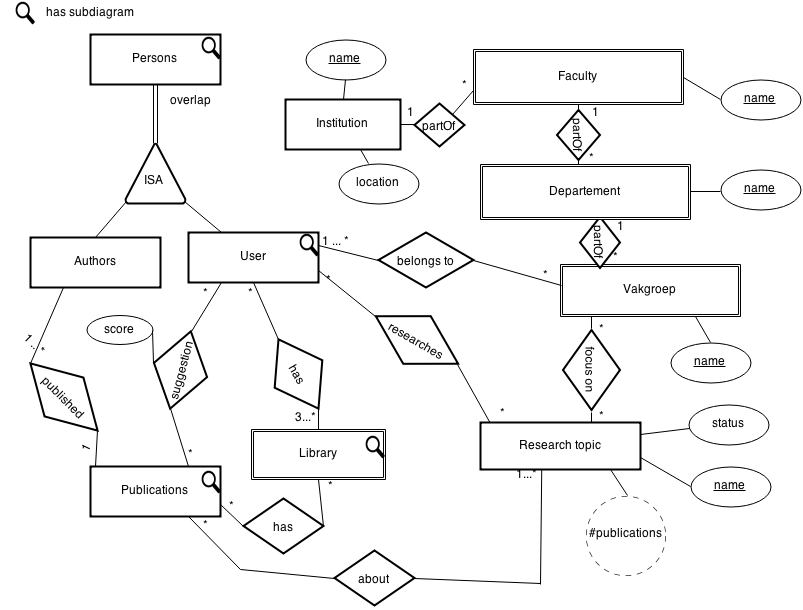
\includegraphics[width=149mm]{minimised_er_diagram_v3.png}
 \caption{Geminimaliseerde structuur van de graf in een (E)ER-model}
 \label{ER-model}
\end{figure}

Dit is een overzicht van het algehele model van de database, de entiteiten met een vergrootglas worden gedetailleerder toegelicht in hun bijhorende subdiagrammen.\\

\subsection{Gebruikers \& affiliatie}

De database is zodanig gemodelleerd dat we in staat zijn van de affiliatie van personen bij te houden en later te gebruiken om mensen in eenzelfde departement of faculteit met elkaar in contact te kunnen brengen. Verder zou dit van pas kunnen komen bij het genereren van lees-suggesties. De key voor een "'Institution"', "'Faculty"', "'Department"' of "'Vakgroep"' bestaat uit het eigen attribuut naam en de entiteit waarmee ze is verbonden als \textit{weak entity set}.\\

\begin{figure}[!h]
\centering
 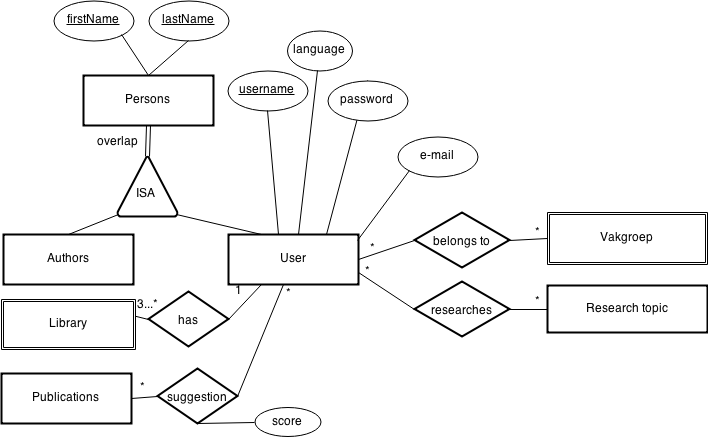
\includegraphics[width=145mm]{user_diagram.png}
 \caption{Structuur van de "'User"' entiteit}
 \label{User-model}
\end{figure}

%already long enough ;)
Dit diagram geeft een gedetailleerde kijk op de "'User"' entiteit. deze entiteit stelt de gebruiker voor en heeft 2 unieke keys: zijn "'username"' en de "'firstName"', "'lastName"' combo die ge\"erfd wordt van "'Persons"'. De User heeft geen directe relatie met een publicatie, interactie gebeurt via de "'Library"'.

\subsection{Publicaties}

\begin{figure}[!h]
\centering
 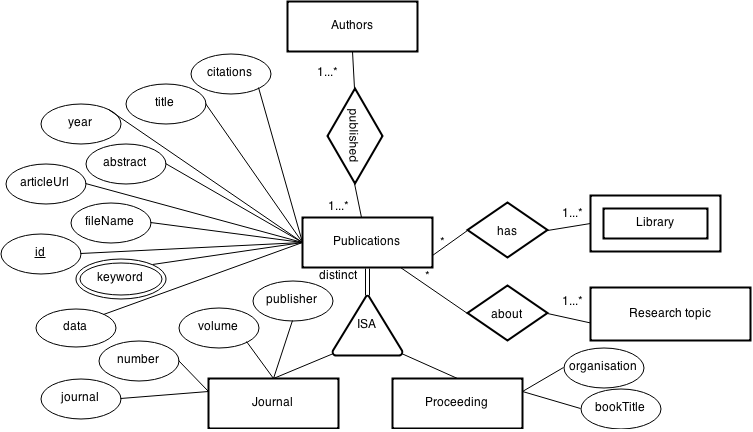
\includegraphics[width=145mm]{publication_diagram.png}
 \caption{Structuur van de "'Publication"' entiteit}
 \label{Publication-model}
\end{figure}

De "'Publication"' entiteit is uitgebreid in deze iteratie met meer attributen. Als key zal er een id worden gebruikt. Het eigenlijke publicatie bestand bevindt zich ook in de database zelf als BLOB, en wordt in dit diagram voorgesteld met het "'data"' attribuut.

"'Publications"' is verder uitgebreid met de subklassen "'journal"' en  "'proceeding"', om de verschillen correct te kunnen modelleren.

\subsection{Bibliotheken}

Onderstaand diagram geef inzicht in de "'Library"' entiteit, in de applicatie zal een gebruiker verschillende bibliotheken kunnen aanleggen om gekozen publicaties in te bewaren en te groeperen. 
\begin{figure}[!h]
\centering
 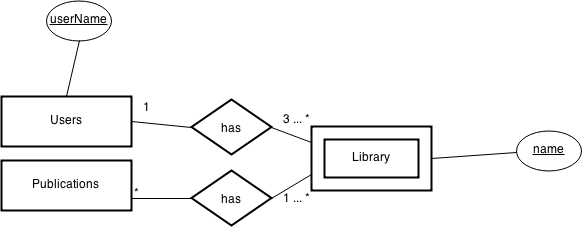
\includegraphics[width=145mm]{library_diagram.png}
 \caption{Structuur van de "'Library"' entiteit}
 \label{Library-model}
\end{figure}

Een gebruiker zal altijd drie vaste bibliotheken hebben:

\begin{description}

\item[Uploaded] Alle publicaties die de gebruiker toevoegt komen automatisch in deze bibliotheek terecht

\item[Portfolio] Hierin kan de gebruiker publicaties toevoegen waaraan hij heeft meegewerkt of die hij zelf heeft geschreven. Het is als het ware zijn uithangbord naar andere gebruikers toe.

\item[Favorites] Daarnaast kan hij ook een eigen collectie met publicaties van derden aanleggen op basis van zijn interesses in deze bibliotheek.

\end{description}

Libraries vormen een zwakke entiteit en hebben als key een naam en de gebruikersnaam van de eigenaar. Bijgevolg kan een gebruiker dus niet meerdere bibliotheken met dezelfde naam aanmaken. \\

\clearpage

\section{Component Design}
\label{sec:components}

In dit gedeelte worden de verschillende componenten die samen de applicatie vormen, verder toegelicht. Onderstaand klassediagram geeft een overzicht van deze componenten. Merk op dat hierin enkel belangrijke klassen, attributen en associaties zijn gemoddeleerd. Gedetailleerde informatie omtrent types e.d. zijn weggelaten indien overbodig. 

\begin{figure}[!h]
\centering
 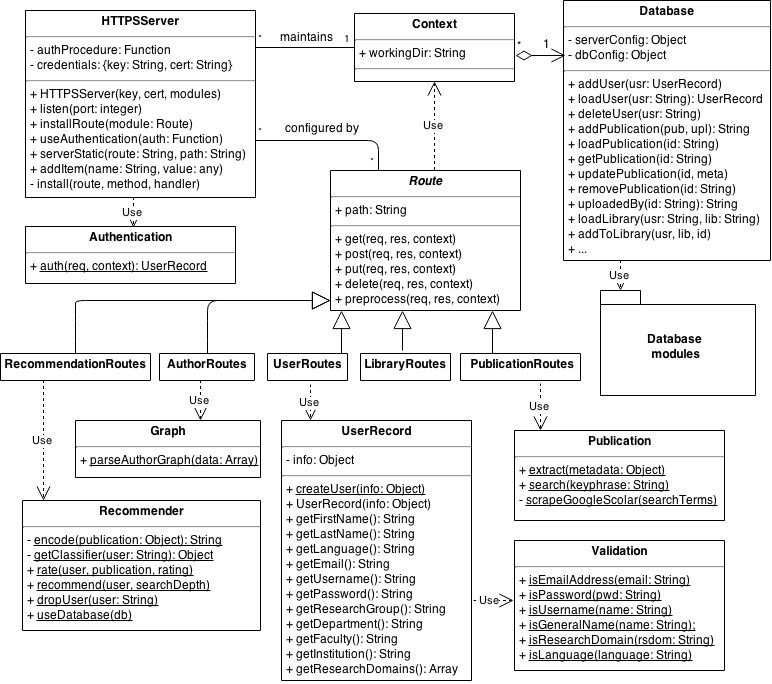
\includegraphics[width=160mm]{Klassediagram.png}
 \caption{UML-klassediagram van de verschillende componenten }
 \label{class-diagram}
\end{figure}

\subsection{Server}

De server zelf vormt het ingangspunt van de server-tier. Deze module kan geconfigureerd worden met bepaalde routes en zal zo de request naar een bepaalde handler delegeren (met de bedoeling om zo een RESTFul API samen te stellen). De handlers zullen op hun beurt dan weer gebruik maken van de back-end, waar de meeste applicatielogica van de server-tier zich bevindt en waar ook de communicatie met de DB-tier plaatsvindt.  \\

Momenteel bevat dit component vooral methodes om de server te configureren en om ze op te starten met een SSL-certificaat (HTTPS). Daarnaast is er ook een mogelijkheid voorzien om de server te configureren met extra modules en om authenticatie toe te voegen aan bepaalde requests.

\subsection{Routes}

Routes zullen op de server worden gebruikt om de verschillende requests af te handelen.Op die manier wordt het configureren van de Server API gebruiksvriendelijker en overzichtelijker in de code. Routes kunnen gemakkelijk worden gedefinieerd en bevinden zich in de folder \textit{/server/routes}.\\

Een bepaalde route wordt gekenmerkt door een bepaald path (zoals /users) en verschillende handlers voor zowel GET, POST, PUT \& DELETE requests op die route. Een handler is hierbij een functie die een request en response als argumenten nemen en het response-object correct configureert op basis van de request. Een route-object ondersteunt dan properties \textit{get}, \textit{post)}, ... om deze handlers te gebruiken. Een opsomming van de ge\"implementeerde routes is terug te vinden in sectie~\ref{api}.

\subsection{Authentication}

Deze module bevat een speciale functie die aan de hand van het HTTP-request zal bepalen welke user zich hier authenticeert (of hij geeft aan dat de credentials ongeldig zijn). Specifiek wordt hier gebruik gemaakt van Basic Authentication, waarbij de gebruiker zijn username:password over HTTPS meegeeft aan de server, ge\"encodeerd in base64.\\

Vervolgens kan men dan gebruik maken van de methode \textit{useAuthentication} van de server om deze module te gebruiken authenticatie. Routes kunnen vervolgens aangeven of een geauthenticeerde gebruiker al dan niet toestemming heeft om een bepaalde request uit te voeren. Dit kan door aan de handlers een speciale property \textit{auth} mee te geven. Op die manier wordt het gemakkelijk om een handler te beveiligen, wordt code-duplicatie vermeden en kan men gemakkelijk van authenticatiestrategie veranderen.

\subsection{Validation}

Deze module wordt niet alleen op de back-end, maar ook op de front-end gebruikt om input van de gebruiker te valideren. Server-side validation is niet alleen aangewezen vanuit een design-standpunt, maar is ook noodzakelijk om veiligheidsredenen. Client-side validation zorgt dan weer voor een aangenamere en effici\"entere gebruikerservaring. \\

Concreet gaat hier in deze module vooral om functies die worden gebruikt om de geldigheid van een gebruikersnaam, wachtwoord, e-mailadres etc. te controleren. Zo zal men in deze module procedures zoals \textit{validUsername(username)}, \textit{validPassword(pwd)}, ... terugvinden. Dit gebeurt aan de hand van regular expressions, die standaard worden aangeboden door JavaScript. Daarnaast wordt ook een aparte module \textit{researchDomain} gebruikt, waarin mogelijke onderzoeksdomeinen en disciplines, onderverdeeld in majors en minors, wordt geraadpleegd om na te gaan of het opgegeven onderzoeksdomein wel bestaat.

\subsection{UserRecord}

Deze klasse bevat alle noodzakelijke informatie over een bepaalde gebruiker in het systeem. Zo'n gebruikersinformatie kan ofwel worden geladen uit de database, ofwel kan via een constructor een nieuwe gebruiker worden aangemaakt die eerst alle input zal valideren en het wachtwoord zal hashen.

Het resulterende object kan dan gebruikt worden om gemakkelijk gegevens van de gebruiker op te vragen, of men kan aan de database een nieuw UserRecord geven om aan het systeem toe te voegen. Ook bij het laden van user zal de database zo'n object teruggeven. Naast de gebruikelijke kenmerken zoals (gebruikers)naam, taal, e-mailadres houdt dit record ook de affiliatie en onderzoeksdomeinen van de gebruiker bij.

\paragraph{Opmerking}
Veel van de ge\"exporteerde methodes in deze module zijn asynchroon en verwachten dus een callback bij oproep. Dit patroon zal ook in andere modules (zoals dat van de database) voorkomen en is inherent aan web-applicaties in NodeJS. Bij het laden van de gebruiker uit de database via \textit{loadUser(db, name, callback)} zal zo bijvoorbeeld niet meteen een nieuw gebruikersobject worden aangemaakt, maar zal de meegeleverde callback worden opgeroepen met de gebruikersinfo als deze is geladen. 

\subsection{Publication}

Een aparte module is op de back-end voorzien om meer informatie op te halen van publicaties, gebaseerd op externe bronnen (meer bepaald Google Scholar). Hiervoor wordt gebruik gemaakt van een techniek die \textit{web scraping} heet. Daarbij wordt aan de hand van de juiste HTTP-request en URL de resulterende HTML gebruikt om informatie van het web te halen indien er geen API beschikbaar is. Voor de scraping zelf wordt gebruik gemaakt van de library Cheerio~\cite{website:cheerio}. \\

Zo biedt SKRIBL de mogelijkheid om metadata van een publicatie te laten aanvullen met deze informatie van Google Scholar. Concreet wordt voor deze extractie verwacht dat de gebruiker een metadata-object voorziet met daarin minstens de titel van de publicatie. Aan de hand van die gegevens zal deze module dan extra informatie opzoeken om de metadata verder aan te vullen met bijkomende attributen. \\

Daarnaast wordt de scraping ook gebruikt om zoekresultaten te verzamelen, gebruik makende van een bepaalde keyphrase. Opnieuw wordt hiervoor beroep gedaan op de zoekfunctionaliteit van Google Scholar en worden de hoogst gerankte resultaten voor de zoekterm teruggegeven.

\subsection{Graph}

Om meteen een overzicht te hebben van de relaties tussen verschillende auteurs, kan de gebruiker de co-auteurrelaties (en hun bijhorende publicaties) laten visualiseren in een graph. Aangezien de gebruikte database, OrientDB, (onder andere) een graph-database is, kan men relatief eenvoudig deze overlopen om dergelijk graph te construeren. \\

Deze module zorgt voor de omzetting van de gegevens uit de database (na een traversal) naar een formaat met dat op de front-end kan worden gevisualiseerd. Zo vindt men hier een functie \textit{parseAuthorGraph(data)} terug, die deze informatie zal omzetten naar een JSON-representatie met vertices \& edges.

\subsection{Recommender}

Om gemakkelijk nieuwe publicaties te ontdekken, laat SKRIBL gebruikers toe om aangerade publicaties op te vragen, gebaseerd op gepersonaliseerde voorkeuren van de gebruiker. Om deze voorkeuren aan te leren, wordt gebruik gemaakt van een Naive Bayesian Classifier. Deze zal onder andere de titel, abstract \& keywords van een publicatie analyseren voor de classificatie. \\

Concreet kan een gebruiker, gebruik makende van de functie \textit{rate}, een publicatie ofwel een positieve of negatieve score toekennen. Dit zal bijvoorbeeld gebeuren wanneer hij/zij op de (dis)like-knop klikt, alsook wanneer de publicatie wordt toegevoegd aan de Favorites-library. Op die manier kan de classifier per gebruiker worden getrained om later voorspellingen te maken over de beoordeling van ongeziene publicaties.

Wanneer dan vervolgens de recommendations worden opgevraagd met de gelijknamige functie, zal er eerst beroep worden gedaan op de database. Vermits deze georganiseerd is als graph, is het mogelijk om alle publicaties die (graphsgewijs) dicht bij de gebruiker liggen op te vragen, rekening houdend met hun impact/aantal views. Vervolgens wordt de classifier dan gebruikt om in deze set van publicaties de beoordeling van de gebruiker te voorspellen. Publicaties die dan negatief geclassificeerd worden, worden verwijderd uit de lijst. \\

Ten slotte kan men in deze module ook nog een cache terugvinden. Deze wordt gebruikt om performantie te verbeteren bij het herhaaldelijk inladen en wegschrijven van de classifier. Concreet wordt er gewerkt met een \textit{Least-recently used} (LRU) cache die wijzigingen meteen doorvoert in de database \textit{(write-through)}.

\subsection{Database}

In deze module vindt men een abstractie voor alle communicatie met de database. Het implementeert een bepaalde interface die onder andere door de Server- en UserInfo-modules wordt verwacht. Concreet is het Database-object verantwoordelijk voor het opzetten van een databaseverbinding en het uitvoeren van de nodige queries voor de interactie met het model. Zo worden er methodes aangeboden die onder andere nieuwe gebruikers toevoegen, gegevens van bestaande gebruikers opvragen of een nieuwe publicatie opslaan.\\

Om de code hiervoor te organiseren, zijn er voor elke entiteit aparte modules gemaakt die aan de database kunnen worden toegevoegd en die verantwoordelijk zijn voor een bepaald deel van haar functionaliteit. Op die manier wordt vermeden dat deze klasse onoverzichtelijk veel code op zich moet nemen en kan men gemakkelijk een bepaald deel van de databaselogica terugvinden. \\

Ten slotte bevat de database ook redelijk wat private methodes; deze zijn nodig om alle gegevens correct op te slaan volgens het (E)ER-diagram uit figuur~\ref{ER-model}. Zo worden in de database ook al alle lagen van de affiliation (researchGroup, department, faculty, institution) correct bijgehouden. Op dezelfde manier worden ook researchDomains gemodelleerd op de database als aparte entiteiten.\\

De communicatie met de server waarop de database zich bevindt, gebeurt aan de hand van een binary protocol dat OrientDB aanbiedt. Hiervoor wordt gebruik gemaakt van de open-source library Oriento, zodat de queries gewoon kunnen worden uitgevoerd vanuit JS. \\

Database transacties zijn ge\"implementeerd en zorgen ervoor dat kans op corruptie van de database tot een minimum wordt beperkt en de data van de gebruikers verder wordt beschermd. Het is dan ook cruciaal dat men voor dit soort van applicatie, zowel tijdens development als bij de oplevering, op een consistente database kan rekenen.

\clearpage

\section{Software domain design}

In dit onderdeel wordt bekeken hoe de verschillende componenten in het systeem samenwerken om een bepaalde functionaliteit te verwezenlijken. Op die manier wordt duidelijk gemaakt welke verantwoordelijkheid elk onderdeel in het systeem heeft.
Meestal zal de beschrijving worden gegeven aan de hand van een sequentiediagram of (in het geval van een algoritme) pseudocode.

Voor een volledig overzicht van alle benodige functionaliteit wordt verwezen naar het SRS \cite{Xtreport:SRS}.

\subsection{Inloggen}

Bij het inloggen zal de client eerst een request sturen naar de server met gebruikersnaam en wachtwoord toegevoegd in plaintext. Indien correct, zal de server een id-string terugsturen naar de client die hij later bij elke request die authenticatie vereist moet toevoegen. Volgens de principes van een RESTful ontwerp, mag er echter geen (session) state op de server worden bijgehouden en zal deze unieke identificatiestring dus niet gebonden zijn aan een bepaalde sessie. Momenteel is het gewoon een encodering van de gebruikersnaam en wachtwoord in base64 (= Basic Access Authentication).
Uit veiligheidsoverwegingen zal voor de persistente opslag van wachtwoorden in de databasenk wel encryptie worden gebruikt. \\ 

Uit deze beschrijving kunnen we ook al afleiden dat het zeker nodig zal zijn HTTPS te gebruiken om zo alle communicatie tussen client en server te encrypteren met SSL (weliswaar met een self-signed key). Zoniet zou het niet veilig zijn om wachtwoorden (ge\"encodeerd of niet) door te sturen.

\begin{figure}[!h]
\centering
 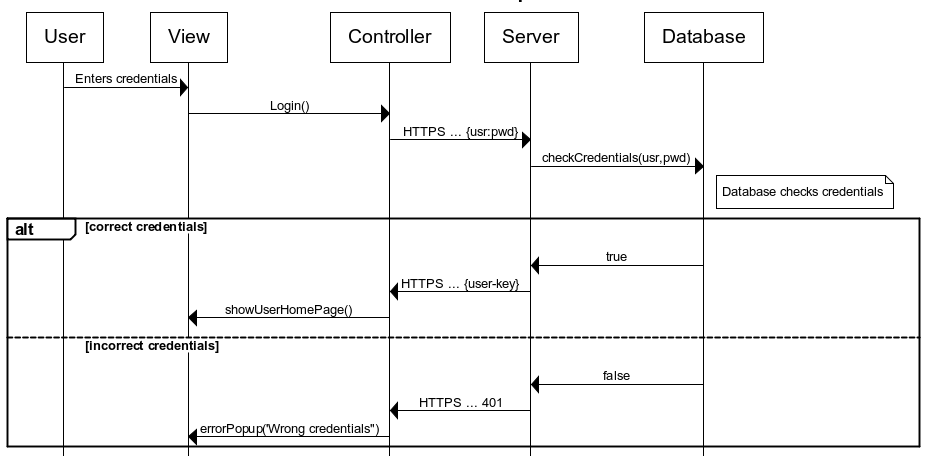
\includegraphics[width=145mm]{login-sequence.png}
 \caption{Vereenvoudigd sequentiediagram bij het inloggen}
 \label{login-sequence}
\end{figure}

\paragraph{Opmerking}

Bovenstaand sequentiediagram is slechts een vereenvoudiging van wat er in werkelijkheid gebeurt, zo zijn bijvoorbeeld procedures zoals checkCredentials in werkelijkheid asynchroon, en zullen ze dus geen boolean teruggeven, maar werken ze met callbacks.

Deze opmerking geldt ook voor alle andere sequentiediagrammen in dit onderdeel.

\subsection{Registreren}

Om een nieuwe gebruiker te registeren, dient men eerst een registratieformulier in te vullen. Om de gebruikerservaring hierbij de verbeteren zal dit gebeuren met client-side validation (naast de server-side validation, die noodzakelijk is). 

Van zodra alle informatie is ingevuld, zal de client een identificatiestring terugkrijgen indien de nieuwe gebruiker succesvol is toegevoegd. Zoniet, zal de server een HTTP 40x-error teruggeven.

\begin{figure}[!h]
\centering
 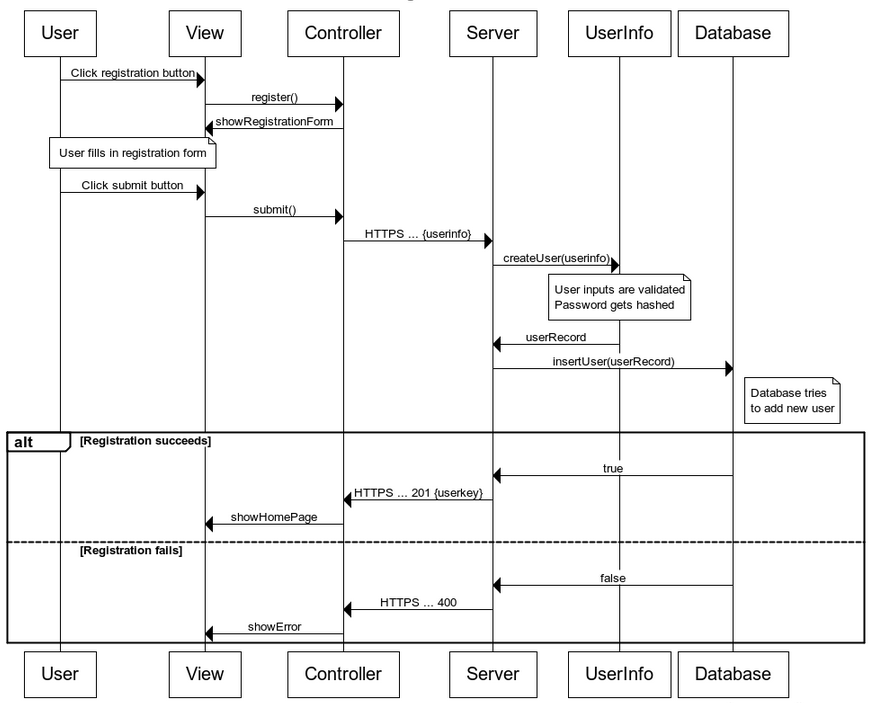
\includegraphics[width=145mm]{registration-sequence.png}
 \caption{Vereenvoudigd sequentiediagram bij het registreren}
 \label{register-sequence}
\end{figure}

\subsection{Publicaties toevoegen}

Een nieuwe publicatie toevoegen gebeurt door een combinatie van de HTTP PUT, GET en POST commando's. Eerst en vooral dient men de publicatie zelf te uploaden met HTTP PUT. Dit kan zowel met een URL als via een traditionele upload. De server zal aan de hand van dit bestand dan een nieuwe publicatie aanmaken in de database met een bepaald id, dat aan de client wordt teruggegeven. \\

Bij SKRIBL hebben we ervoor gekozen om vervolgens automatisch metadata te laten aanvullen aan de hand van een GET-request met dit id (en query-parameter `extract'). Dit is niet verplicht (third-party developers kunnen deze stap en de bijhorende request overslaan), maar de keuze om sowieso metadata te extraheren via scraping bespaart over het algemeen veel typwerk en zorgt dus voor een betere gebruikerservaring. \\

Vervolgens kan de gebruiker deze voorgestelde metadata bekijken en aanpassen indien nodig. Van zodra alle wijzigingen zijn aangebracht, kan de JSON met de ingevulde gegevens worden doorgestuurd aan de hand van een POST-request. \\

Hieronder volgt een sequentiediagram die dit proces illustreert. Om het overzicht te bewaren, werden mogelijke foutmeldingen niet gemodelleerd:

\begin{figure}[!h]
\centering
 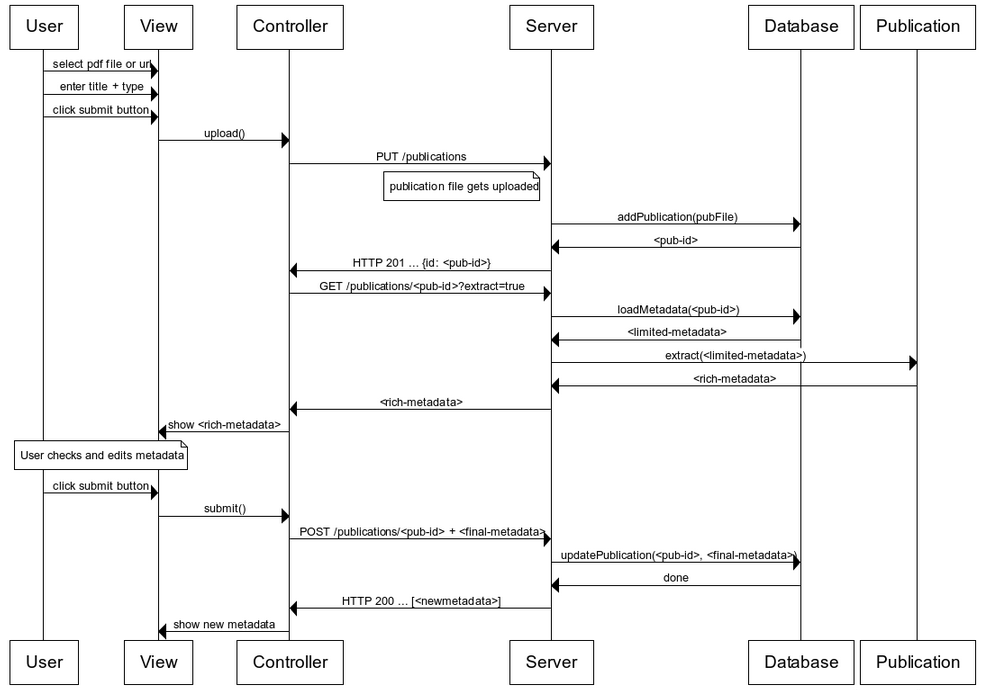
\includegraphics[width=165mm]{upload-sequence.png}
 \caption{Vereenvoudigd sequentiediagram bij het toevoegen van publicaties}
 \label{upload-sequence}
\end{figure}

Daarnaast dient men bij een upload ook nog volgende stappen uit te voeren:

\begin{itemize}

\item Voor het uploaden dient men te na te kijken of er nog geen publicatie bestaat met dezelfde titel \& type om duplicaten te vermijden. Dit kan aan de hand van de zoekfunctionaliteiten in de server API (cf. GET /publications \& POST /publications). Indien de publicatie al bestaat, kan de gebruiker hem gewoon toevoegen aan een van zijn bibliotheken in plaats van hem opnieuw te uploaden.

\item Hetzelfde geldt ook voor auteurs: om publicaties te linken aan bestaande auteurs kan men via de zoekfunctie op naam (cf. GET /authors) gekende auteurs en enkele van hun publicaties opvragen. In het geval dat de auteur een SKRIBL-gebruiker is, kan zelf zijn/haar hele profiel eerst worden geraadpleegd. Indien uiteindelijk wordt besloten dat het om dezelfde auteur gaat, dient men zijn/haar id (uit de zoekresultaten) mee te geven bij de POST request.

\end{itemize}

\subsection{Zoeken naar publicaties}

Dit scenario illustreert hoe men ook meteen op zoek kan gaan naar reeds bestaande publicaties. De search aan de hand van een keyphrase (cf. GET /publications) wordt hier besproken, op een gelijkaardige manier zou men ook de geadvanceerdere versie (cf. POST /publications) kunnen gebruiken. \\

Bij het zoeken worden zowel interne als externe resultaten teruggegeven. Interne resultaten krijgen een titel, type, id en lijst van auteurs mee om meteen een korte samenvatting te geven van elke publicatie. Aan de hand van het id kan men dan meer informatie opvragen of de publicatie toevoegen aan een van zijn/haar bibliotheken. \\

\begin{figure}[!h]
\centering
 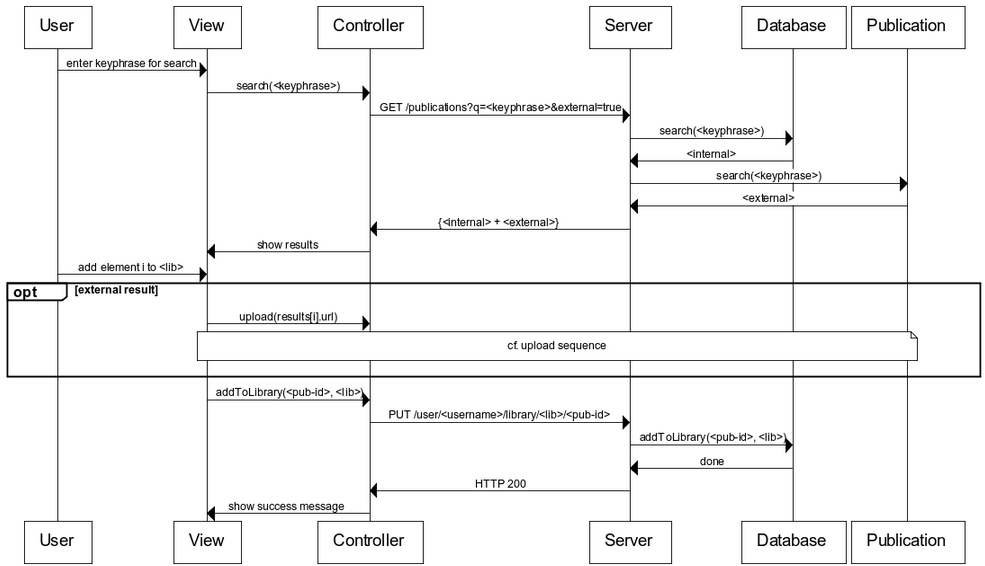
\includegraphics[width=140mm]{search-sequence.png}
 \caption{Vereenvoudigd sequentiediagram bij het zoeken naar publicaties}
 \label{upload-sequence}
\end{figure}

Externe resultaten van Google Scholar dragen op een gelijkaardige manier al meteen redelijk wat metadata mee en bevatten ook een download-link (indien beschikbaar) naar de publicatie in kwestie. Deze kan men dan ook meteen gebruiken om de publicatie toe te voegen aan het systeem en vervolgens aan een van zijn/haar bibliotheken.

\subsection{Bibliotheek weergeven}

Een gebruiker kan publicaties groeperen in verschillende bibliotheken. Standaard zijn "Portfolio", "Uploaded" \& "Favorites" sowieso aanwezig wanneer men zich registreert op SKRIBL. \\

Een bibliotheek kan worden geladen door gebruik te maken van een GET-request. Dit zal een array met ids teruggeven van alle publicaties in die bibliotheek. Vervolgens kan een lijst met uitgebreide info van elke publicatie worden weergegeven door de metadata op te halen aan de hand van hun ids (cf. API in sectie ~\ref{api}).

Aangezien de metadata momenteel niet zo uitgebreid is en de lijst de meeste info inline kan bevatten, is deze methode niet zo ineffici\"ent. Indien het overzicht enkel de titels zou bevatten en de volledige metadata veel uitgebreider zou zijn, kan men naast de ids in deze request ook al meteen de titels meegeven om zo extra communicatie tussen client \& server te vermijden. \

Onderstaand sequentiediagram illustreert dit proces. Daarnaast toont het ook aan hoe een gebruiker een publicatie uit de lijst kan downloaden.

\begin{figure}[!h]
\centering
 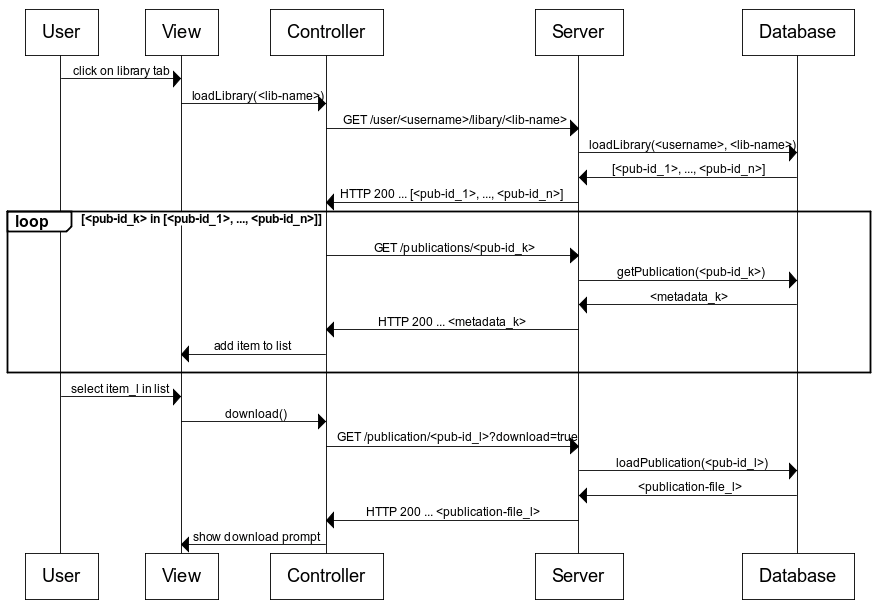
\includegraphics[width=142mm]{library-sequence.png}
 \caption{Vereenvoudigd sequentiediagram bij het laden van een bibliotheek}
 \label{library-sequence}
\end{figure}

\subsection{Publicaties aanraden}

SKRIBL laat ook toe om aan gebruikers nieuwe publicaties aan te raden op basis van eerder vastgelegde voorkeuren. Zoals reeds vermeld, wordt hiervoor gebruik gemaakt van een Naive Bayesian Classifier die probeert te voorspellen of een publicatie al dan niet interessant is voor de gebruiker.

Deze voorkeuren worden vastgelegd op twee verschillende manieren. Eenerzijds kan de client een bepaalde request gebruiken om een rating aan een publicatie mee te geven. Anderzijds zal een publicatie automatisch als een positief voorbeeld worden geregistreerd indien deze wordt toegevoegd aan zijn/haar Favorites-library. \\

Het idee achter het bijhouden van classifiers werd al besproken in de vorige sectie~\ref{sec:components}. Om nu zelf nieuwe publicaties te ontdekken wordt gebruik gemaakt van de graph-structuur in de database. Deze zal, vertrekkend vanuit de gebruikers-node, alle publicaties op een bepaalde afstand in de graph aanduiden als mogelijke kandidaten voor de aan te raden publicaties. Hierdoor zullen automatisch alle publicaties bereikbaar vanuit de gebruiker zijn bibliotheken (waaronder dus ook de favorieten) en onderzoeksdomeinen in aanmerking komen. De resultaten worden dan gesorteerd op hun impact (gebaseerd op het aantal views).

Vervolgens worden de geselecteerde publicaties gefilterd door de classifier. Deze zal proberen om oninteressante publicaties voor de gebruiker er meteen uit te halen door onder andere de tekst van de titel, abstract en keywords te analyseren. Zo wordt bijvoorbeeld vermeden dat een publicatie die reeds werd afgekeurd door de gebruiker (of een gelijkaardige publicatie) opnieuw opduikt in de lijst met recommendations.

\begin{figure}[!h]
\centering
 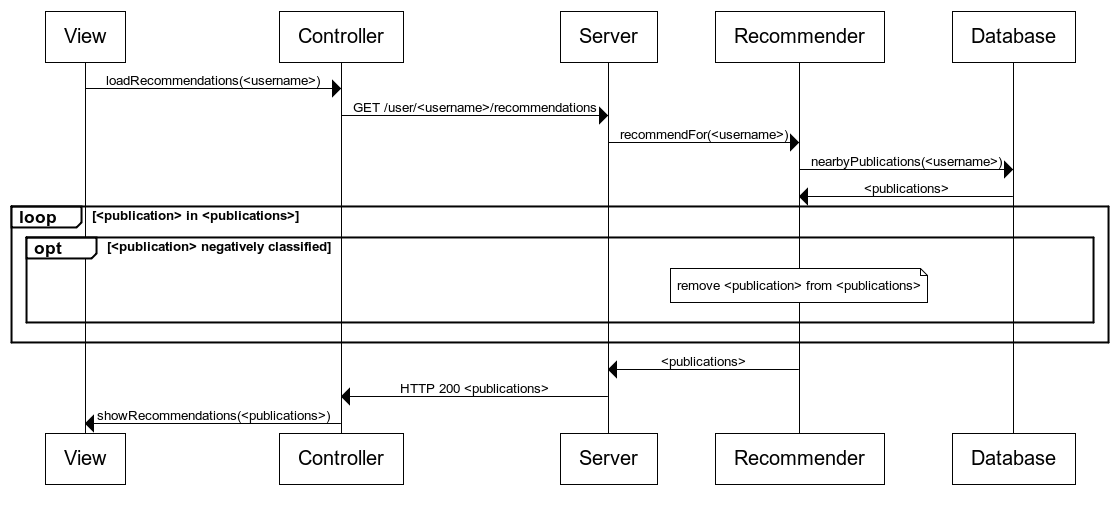
\includegraphics[width=145mm]{recommendations.png}
 \caption{Vereenvoudigd sequentiediagram bij het aanraden van een bibliotheek}
 \label{recommendation-sequence}
\end{figure}

\clearpage

\section{Human Interface Design}

\subsection{Inleiding}

Met het ontwikkelen van de grafische user interface (GUI) wordt getracht een narratief te bereiken dat sterk visueel is, doch niet in de weg komt te staan van de beoogde functionaliteit. In het algemeen dient de sfeer neutraal en professioneel ervaren te worden, maar er wordt tevens getracht afstand te nemen van klassiek-wetenschappelijke visuele identiteiten. Doorheen dit document wordt met GUI zowel de User Experience (UX) als de User Interface (UI) bedoeld om de communicatie erover zo simpel mogelijk te houden.


\subsection{Principes}

De reden om überhaupt aandacht te schenken aan de implementatie van `goed (grafisch) ontwerp' is de overtuiging dat deze het product gebruiksvriendelijker maakt. Verder heeft het ontwerp als doel het product begrijpbaar te maken. Vanuit dit idee is het zinvol om na te denken hoe het unieke concept van onze applicatie zich grafisch kan vertalen. Een verhaal eindigt met andere woorden niet louter bij het systeem-ontwerp in al zijn facetten, maar ook de esthetiek van de applicatie en gebruikservaring van de consument ten aanzien van deze applicatie zijn relevant. %Het zijn de twee zijden van eenzelfde munt.
\\

Aangezien SKRIBL zich wendt tot meerdere platformen is de responsiviteit van cruciaal belang. Zo wordt er verder gekeken dan louter het schalen van visuele elementen, maar ook naar de manier van interactie. Een voorbeeld hiervan is het gebruik van grotere knoppen bij het ontwerpen voor een mobiel platform ten opzichte van hyperlinks bij een desktop computer. Een uitgewerkt voorbeeld hiervan kan geraadpleegd worden in appendix B. Het spreekt voor zich dat ook de functionaliteit per platform verschillend is. In het algemeen kan gesteld worden dat elementen die een hogere vorm van kernfunctionaliteit bevatten, ook de voorrang krijgen bij het toepassen van herschalingen.
\\

We trachten een grafische interface te creëren waarbij een gebruiker intuïtief de functie van ieder element aanvoelt. Hierbij wordt er waar mogelijk met symbolen en iconen gewerkt met als doel een zelf-verklarende ervaring. In een ideale situatie zou het gebruik van de UI/UX getest worden met behulp van `usability tests' met verschillende doelgroepen. Hoewel de relevantie en de noodzakelijkheid hiervan niet te ontkennen valt voor een product als SKRIBL, wordt er van uit gegaan dat het testen hiervan buiten de huidige omvang van de opdracht valt.
\\

De grote meester Aristoteles zei ooit over schoonheid dat het iets is waar: “je noch iets aan kunt toevoegen, noch iets uit kunt wegnemen, zonder het geheel te storen”.~\cite{gadamer} Dit wordt door ontwerpers ook wel eens het principe van de interfaceless interface genoemd. Hiermee wordt gedoeld op het streven naar een grafische functionele ervaring zonder dat hier onnodige elementen aanwezig zijn, iets wat SKRIBL ook tracht te realiseren, doch op een speelse manier. 
\\

SKRIBL volgt duidelijk een grafische stijlstroming, namelijk die van Google’s Material Design ~\cite{website:Material}. Materiaal is een metafoor die door Google gebruikt wordt om te duiden op wat ze “gerationaliseerde ruimte” noemen, aangevuld met een systeem van animaties. Een van de belangrijkste elementen om inhoud te visualiseren is het gebruik van virtuele “kaarten”. Hoewel Material Design een recente visuele stroming binnen de UI wereld is, heeft het er alle schijn naar dat het gros van de ideologie zinvol en universeel genoeg is om geen hype te wezen. In het algemeen zijn er twee grote stromingen binnen digitaal ontwerp:

\begin{description}

\item[Flat Design] Alle interfacing elementen worden `digitaal' en vlak wilt behouden zonder referenties te maken naar de niet-virtuele wereld (cfr Windows)

\item[Skeuomorphisme] Het vertalen van niet-virtuele kenmerken in het digitale ontwerp (cfr iOS pre 8.x)

\end{description}

Het gaat voorbij de omvang van dit document om dit uitvoerig te bespreken. Material Design~\cite{website:Material} behoord echter tot het kamp van wat soms “flatty” genoemd wordt; een speelse variant op flat design waarbij skeuomorphistische elementen aanwezig zijn die echter de regels volgen van een verzonnen wereld (ten opzichte van de echte wereld).
\\

Zo worden slagschaduwen gebruikt als visuele metafoor voor diepte. Het doel is deze op zo’n manier aan te wenden dat deze de logische opbouw van de applicatie volgen. In appendix C wordt dit verder duidelijk gemaakt met behulp van een voorbeeld.

\clearpage


\section{Externe API}
\label{api}

Naast de grafische interface, biedt het systeem ook een API aan voor externe ontwikkelaars die hun eigen applicaties willen integreren met SKRIBL. Dit gebeurt met RESTful API over HTTP(S).

\subsection{Gebruikers}

Deze HTTP-requests hebben betrekking tot de gebruikers van het systeem. Ze laten toe om bijvoorbeeld een nieuwe gebruiker te registreren of om met een bestaand profiel in te loggen.

\begin{description}

\item[POST /login] Deze request wordt gebruikt om in te loggen, men geeft de gebruikersnaam en het wachtwoord (over HTTPS) mee in JSON-formaat en krijgt een unieke identificatiestring terug van de server die men later moet meegeven bij bepaalde requests.

\item[GET /user/<username>] Op deze manier kan men in JSON-formaat relevante informatie van een bepaalde gebruiker in het systeem opvragen.

\item[PUT /user/<username>] Met deze request kan een nieuwe gebruiker op de server worden aangemaakt. Alle nodige gebruikersinformatie dient te worden meegegeven bij de request als JSON-data.

\item[DELETE /user/<username>] Hierbij dient men expliciet zijn/haar identificatiestring mee te geven. Het resultaat is dat de aangeduide gebruiker uit het systeem zal worden verwijderd.

\end{description}

\subsection{Publicaties} 

Voor publicaties zijn er ook enkele routes voorzien om bijvoorbeeld nieuwe publicaties toe te voegen, metadata manueel of automatisch aan te vullen of om een query uit te voeren met bepaalde criteria.

\begin{description}

\item[PUT /publications] Hiermee kan men een nieuwe publicatie uploaden in het systeem. Het bestand kan zowel worden aangeleverd via een URL als met een traditionele upload. De server zal bij deze request een uniek id van de publicatie teruggeven. Aan de hand van de identificatiestring zal de uploader automatisch worden ge\"identificeerd.

\item[GET /publications/<pub-id>] Haalt de metadata van een publicatie op met een meegegeven id. Daarnaast kan men in deze route ook extra metadata opvragen van deze publicatie gebruik makende van de query parameter `extract'. In dit geval zal de oorspronkelijke metadata, aangevuld met informatie van Google Scholar worden teruggegeven. Aan de hand van een extra query parameter `download' in de URL kan men deze request ook gebruiken om het bestand zelf te downloaden. 

\item[POST /publications/<pub-id>] Hiermee kan men de metadata van publicaties updaten, deze dient meegeleverd te worden in JSON-formaat. Voor deze operatie dient men zich tevens te authenticeren als oorspronkelijke uploader van de publicatie.

\item[DELETE /publications/<pub-id>] Deze methode zal een publicatie van de server verwijderen. Ook hier dient men zich correct te authenticeren.

\item[GET /publications] Hierbij wordt verwacht dat men een aparte query-string meegeeft om op zoek te gaan naar een bepaalde publicatie. Het resultaat is dan een JSON-array van publicaties die werden gevonden aan de hand van deze keyphrase. Externe zoekresultaten van Google Scholar kunnen ook worden opgezocht met de query-parameter `external'. Zij zullen tevens een url meedragen, zodat de bijhorende publicatie meteen kan worden bekeken of toegevoegd aan SKRIBL.
\textit{bijvoorbeeld: /publications?q=multicore\&external=true}

\item[POST /publications] Gelijkaardig aan de vorige, kan men deze request ook gebruiken om publicaties te zoeken. Het verschil is dat deze versie geadvanceerder is en meer gerichte resultaten kan teruggeven. Hiervoor dient men dan in de body van de request een specifiekere beschrijving van de zoekcriteria mee te geven als JSON.

\end{description}

\subsection{Bibliotheken}

Een gebruiker kan volgende requests gebruiken om bibliotheken van publicaties te beheren. By default is er sowieso een `Uploaded', `Favorites' \& `Portfolio'-bibliotheek. Voor al deze requests dient men zich te identificeren als eigenaar van deze bibliotheek.

\begin{description}

\item[GET /user/<username>/library] Hiermee worden alle bibliotheken van een gebruiker teruggeven met hun naam.

\item[PUT /user/<username>/library/<library-name>] Om een nieuwe library met een bepaalde naam aan te maken.

\item[DELETE /user/<username>/library/<library-name>] Om een bestaande library met een bepaalde naam te verwijderen.

\item[GET /user/<username>/library/<library-name>] Hiermee kan men alle publicaties in een bepaalde library opvragen.

\item[PUT /user/<username>/library/<library-name>/<publication-id>] Om een publicatie met een bepaald id toe te voegen aan een library met een bepaalde naam.

\item[DELETE /user/<username>/library/<library-name>/<publication-id>] Om een publicatie met een bepaald id te verwijderen uit een library met een bepaalde naam.

\end{description}

\subsection{Auteurs}

Extra routes zijn ook voorzien om meer informatie op te vragen omtrent auteurs. Zo kan men bijvoorbeeld een graph opladen om alle coAuteur-relaties van een bepaalde auteur te visualiseren. Ook kan men zoeken op naam en voornaam naar een specifieke auteur met gelijkaardige namen.

\begin{description}

\item[GET /authors] Hiermee kan men op zoek gaan naar auteurs die ongeveer matchen met een bepaalde naam \& voornaam. Deze kunnen respectievelijk worden meegegeven in query-parameters `lastname' \& `firstname'. Het resultaat is dan een JSON array van overeenkomende auteurs met hun id's, volledige namen en enkele van hun publicaties.

\item[GET /authors/<author-id>/publications] Met deze request worden alle publicaties van een auteur met een bepaald id opgelijst in een JSON-array.

\item[GET /authors/<author-id>/graph] Deze request wordt gebruikt om alle co-auteur relaties (en bijhorende publicaties) van een auteur met een bepaald id te visualiseren in een graph. Het resultaat is een JSON die deze graaf encodeert aan de hand van haar vertices \& edges en gevisualiseerd kan worden op de front-end.

\end{description}

\subsection{Ratings \& recommendations}

Ten slotte kan SKRIBL ook per gebruiker voorkeuren aanleren om later nieuwe publicaties aan te raden. Hiervoor moet de gebruiker laten weten of een publicatie al dan niet in de smaak valt. Dit laat toe om dan later een voorspelling te maken voor ongeziene publicaties. Concreet is er dan ook een request voorzien om nieuwe publicaties te ontdekken, gebaseerd op de classificaties afgeleid uit voorgaande beoordelingen.

\begin{description}

\item[GET /user/<username>/recommendations] Hiermee wordt een lijst teruggegeven van publicaties die de gebruiker zouden kunnen interesseren. Om deze lijst op te vragen is basic-authentication vereist. Een parameter 'depth' kan worden meegegeven in de URL om het bereik van de zoekopdracht te beperken.

\item[POST /user/<username>/publication/<pub-id>] Met deze request kan men dan weer laten weten of een publicatie al dan niet de gebruiker aanspreekt. Indien dit het geval is, dient de gebruiker een query-parameter 'like' toe te voegen aan de URL met als waarde 'true'. Zoniet, kan men hetzelfde doen, maar dan met waarde 'false'. Opnieuw dient men zich voor deze request te authenticeren met de credentials van de gebruiker.

\end{description}

\clearpage



% \section{Requirements Matrix}

% Ten slotte kan men in onderstaande tabel terugvinden welke componenten verantwoordelijk % zijn voor welke opgestelde requirement. De codes die hierbij gebruikt worden voor de % requirements zijn afkomstig uit het SRS \cite{Xtreport:SRS}. De verschillende componenten % worden dan weer gerefereerd door hun nummering in sectie ... %insert reference.

%\begin{center}
%\begin{tabular}{|c|c|c|c|c|c|}
% \hline
% \textbf{Requirement} & View/Controller & 5.1 & 5.2 & 5.3 & 5.4 & 5.5\\
% \hline
% FR-U001              &                 &     &     &     &     &   \\
% FR-U002              &                 &     &     &     &     &   \\
% FR-U003              &                 &     &     &     &     &   \\
% FR-U004              &                 &     &     &     &     &   \\
% FR-U005              &                 &     &     &     &     &   \\
% FR-U006              &                 &     &     &     &     &   \\
% FR-U007              &                 &     &     &     &     &    \\
% FR-U008              &                 &     &     &     &     &    \\
% FR-U009              &                 &     &     &     &     &   \\
% FR-U010              &                 &     &     &     &     &   \\
% FR-U011              &                 &     &     &     &     &   \\
% FR-U012              &                 &     &     &     &     &   \\
% FR-U013              &                 &     &     &     &     &   \\
% FR-U014              &                 &     &     &     &     &   \\
% FR-U015              &                 &     &     &     &     &   \\
% FR-U016              &                 &     &     &     &     &   \\
% FR-U017              &                 &     &     &     &     &   \\
% FR-U018              &                 &     &     &     &     &   \\
% FR-U019              &                 &     &     &     &     &   \\
% FR-U020              &                 &     &     &     &     &   \\
% FR-U021              &                 &     &     &     &     &   \\
% FR-U022              &                 &     &     &     &     &   \\
% FR-U023              &                 &     &     &     &     &   \\
% FR-U024              &                 &     &     &     &     &   \\
% FR-U025              &                 &     &     &     &     &   \\
% FR-U026              &                 &     &     &     &     &   \\
% FR-U027              &                 &     &     &     &     &   \\
% \hline
% NFR-S001             &                 &     &     &     &     &   \\
% NFR-S002             &                 &     &     &     &     &   \\
% \hline
%\end{tabular}
%\end{center}

% insert appendices here
%\begin{appendices}
%\section{Appendix A}
%\end{appendices}

\begin{appendices} 
\section{Style Guide}
\subsection{Inleiding en legende}
Het doel van deze style guide is het aanbieden van een aantal duidelijke richtlijnen van de visuele identieit van SKRIBL, dewelke als hulp zal dienen van verdere iteraties, de communicatie en nevenprojecten.
\begin{figure}[!h]
\centering
 
\includegraphics[width=100mm]{pieteruploads/SKRBL_FRNT_Legende.png}
 \caption{De gebruikte legende bij de grafische appendices }
\end{figure}
Doorheen verschillende visualisaties van grafische concepten kunnen iconen voorkomen. Het animatie icoon duid op de aanwezigheid van een animatie, dewelke in combinatie met het interactie-icoon geactiveerd kan worden door een gebruiker. Het laatste icoon duid aan dat deze visuele aspecten identiek zijn als dewelke door Google’s Material Design~\cite{website:Material} geformuleerd worden.

\subsection{Componenten}

Aangezien vele elementen zich rechtstreeks vertalen vanuit Google’s Material Design~\cite{website:Material} is het weinig zinvol alle afzonderlijke componenten in detail te bespreken. Een belangrijk facet aan meerdere componenten is het gebruik van een slagschaduw. Hierbij dient vooral rekening gehouden te worden dat ook in onze wereld de lichtbron zich hoger dan de toeschouwer bevindt. Daardoor zal de slagschaduw zich steevast onderaan het grafisch elementen bevinden wanneer deze “op” het canvas ligt. Wanneer er interactie plaatsvindt met het element in kwestie dient deze schaduw, alsook het kleurenspel, zich hieraan aan te passen. Zo is het aangewezen om een knop ook visueel “in te duwen”, als bevestiging van de interactie voor de gebruiker. Voor het stylen wordt er gebruik gemaakt van een aangepaste versie van MaterializeCSS ~\cite{website:materialize}, hetgeen de snelheid van het ontwikkelen drastisch ten goede komt. Ten slotte wordt er gebruik gemaakt van een dynamisch raster-systeem waardoor de uniformiteit en de responsiviteit gemakkelijk te harmoniëren valt. 

\clearpage

\subsection{Color Palette}
\begin{figure}[!h]
\centering
 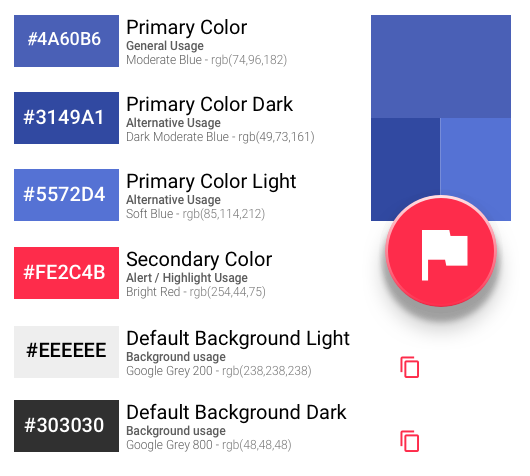
\includegraphics[width=145mm]{pieteruploads/SKRBL_FRNT_ColorPalette.png}
 \caption{De gebruikte kleuren en hun functies}
\end{figure}

Er werd bewust gekozen om slechts enkele zorgvuldig gekozen kleuren te gebruiken bij het ontwerp van de GUI. Het betreft een primaire kleur met twee variaties en een secundaire kleur om speciale gevallen aan te duiden. Verder zijn er twee neutrale kleuren die bepaald werden door Material Design~\cite{website:Material}.

\clearpage

\subsection{Logo}

\begin{figure}[!h]
\centering
 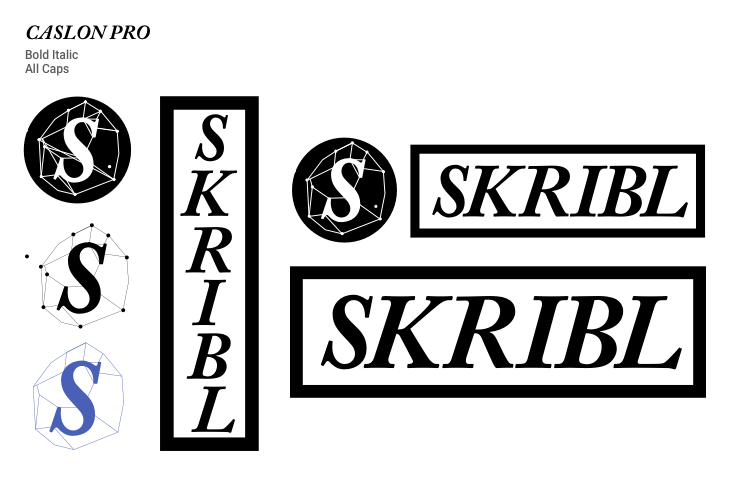
\includegraphics[width=145mm]{pieteruploads/SKRBL_FRNT_Logo.png}
 \caption{Het logo in verschillende variaties}
\end{figure}

SKRIBL heeft een herkenbaar logo dat bestaat uit een schreef-letter. Hierdoor wordt er een knipoog te geven naar het verleden (met de gedrukte tekst), in combinatie met een graf-symboliek die modern oogt. De graf-representatie verhaalt uiteraard ook de sociale factor van de applicatie. De verschillende varianten van het logo worden ingezet op verscheidene gebieden van de communicatie en interfacing. Over het algemeen gezien worden illustraties (vectoren) verkozen boven fotografie (bitmaps) doorheen de ganse applicatie.

\clearpage

\subsection{Typografie}
\begin{figure}[!h]
\centering
 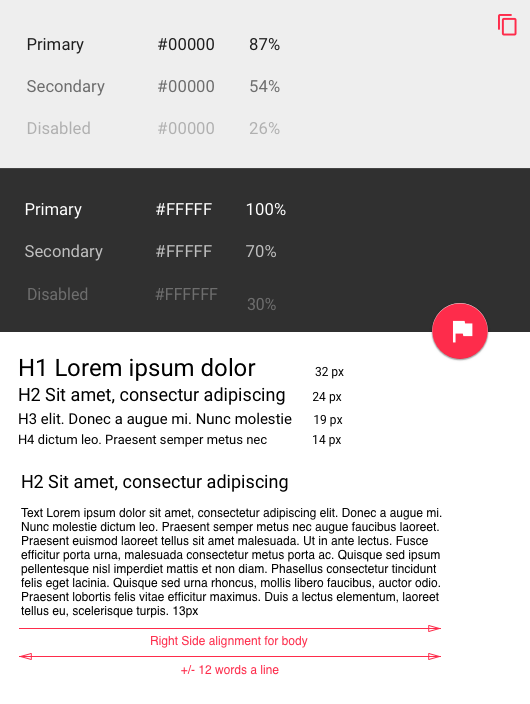
\includegraphics[width=109mm]{pieteruploads/SKRBL_FRNT_typography.png}
 \caption{De typografie in verschillende toepassingen}
\end{figure}

De standaard typografie volgt nagenoeg volledig de suggesties van Material Design~\cite{website:Material} met enkele wijzigingen aan de grootte, interlinie en uitlijning. Het gebruikte font is Roboto. Broodtekst wordt standaard links-uitgelijnd. Dit principe wordt ook op andere facetten van de interface toegepast, namelijk het creëren van heel wat zogenaamde “negatieve ruimte”. Door extra witruimte toe te voegen wordt de simpliciteit verhoogt, hetgeen een rustige en harmonieuze indruk opwekt. Links uitgelijnde tekst ( er wordt gestreefd naar 12 woorden per regel)  wordt in het algemeen gezien als de meest leesbare oplossing.

\clearpage

\section{Wireframe en responsive uitwerking van de landingspagina}

\subsection{Inleiding}
Deze appendix visualiseert de wireframe van de landingspagina tijdens de design-fase. Eenzelfde pagina wordt getoond op een desktop-formaat, een mobiel-formaat en een tablet-formaat. Bij de eerst en laatst genoemde is het logo dat zich bovenaan bevindt interactief en generatief, waarmee bedoeld wordt dat de gebruiker met een steevast uniek logo (op basis van de huidige status van de applicatie) kan interageren.

\clearpage

\subsection{Desktop}
\begin{figure}[!h]
\centering
 
\includegraphics[width=120mm]{pieteruploads/SKRBL_FRNT_Home.png}
 \caption{Visualisatie van de landingspagina }
\end{figure}

\clearpage

\begin{figure}[!h]
\centering
 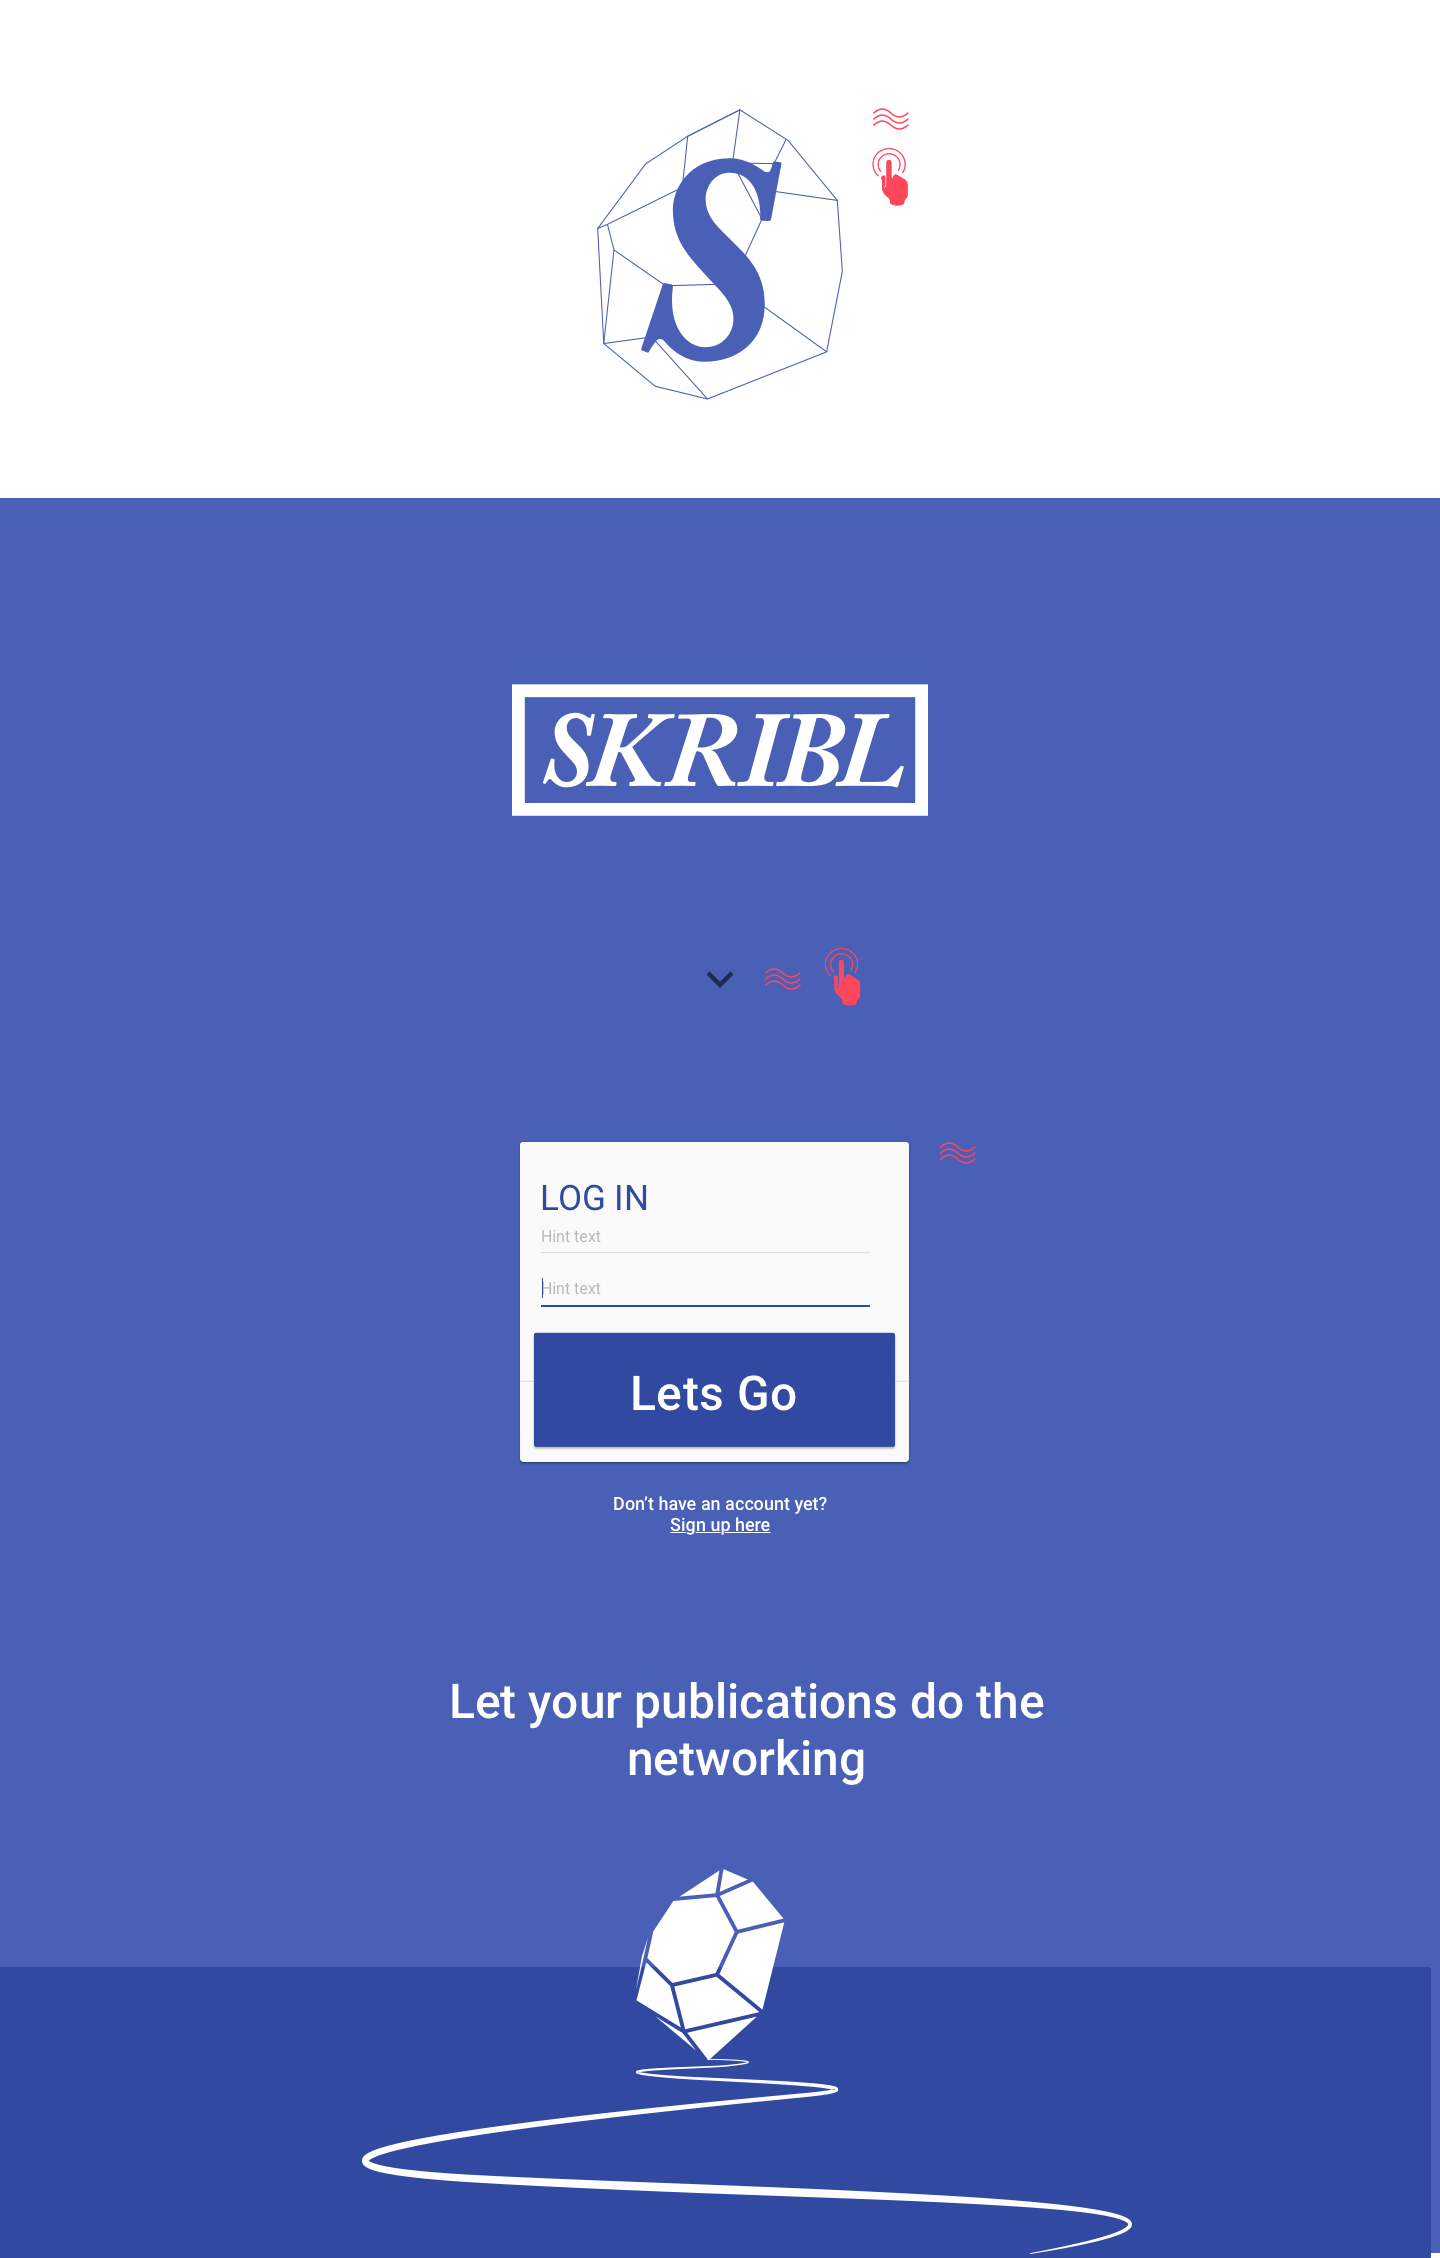
\includegraphics[width=110mm]{pieteruploads/SKRBL_FRNT_Homeafterlogin.png}
 \caption{Visualisatie van de landingspagina bij login}
\end{figure}
\clearpage

\begin{figure}[!h]
\centering
 
\includegraphics[width=80mm]{pieteruploads/SKRBL_FRNT_Homeaftersignup.png}
 \caption{Visualisatie van de landingspagina bij sign up}
\end{figure}
\clearpage


\subsection{Tablet}
\begin{figure}[!h]
\centering
 
\includegraphics[width=100mm]{pieteruploads/SKRBL_FRNT_TabletPortrait.png}
 \caption{Visualisatie van de landingspagina op tablet }
\end{figure}
\clearpage


\subsection{Mobile}
\begin{figure}[!h]
\centering
 
\includegraphics[width=40mm]{pieteruploads/SKRBL_FRNT_MobilePortrait.png}
 \caption{Visualisatie van de landingspagina op mobile }
\end{figure}

\begin{figure}[!h]
\centering
 
\includegraphics[width=40mm]{pieteruploads/SKRBL_FRNT_MobilePortrait2.png}
 \caption{Visualisatie van de landingspagina op mobile na login }
\end{figure}
\clearpage



\section{Mogelijke uitbreidingen}

\subsection{Inleiding}

Deze appendix visualiseert nog twee concepten die onze visie voor SKRIBL op langere termijn projecteren. Door de beperkte tijdsduur van het project werden deze echter niet meer ge\"implementeerd. \\

De meest radicale is waarschijnlijk de implementatie van een simpele command line interface (cli). Het doel hiervan is om een element aan te bieden dat tekstuele interactie met de applicatie mogelijk maakt vanuit het webplatform. Het spreekt voor zich dat deze interactie zich uitsluitend richt op de desktop variant van de applicatie. Het doel ervan is dat de grafische elementen van de interface (zoals bijvoorbeeld de visualisatie van een graf) interactief aangepast wordt door het gebruik van de CLI. 

Verder wordt het gebruik van het navigatie-menu getoond (de statische balk bovenaan), alsook het functie-menu. Deze laatste, dewelke ook statisch is, biedt een aantal specifieke functies aan ten behoeve van de huidige viewport. Hiermee wordt bedoeld dat de functies in kwestie context-gebonden zijn; zo zal een gebruiker via deze weg zijn profiel kunnen aanpassen wanneer hij zich op de profiel pagina bevindt. Ten slotte wordt een eerste aanzet gegeven naar hoe een bepaalde datavisualisatie er uit kan zien binnen de applicatie.


\clearpage
\subsection{Dashboard and CLI}
\begin{figure}[!h]
\centering
 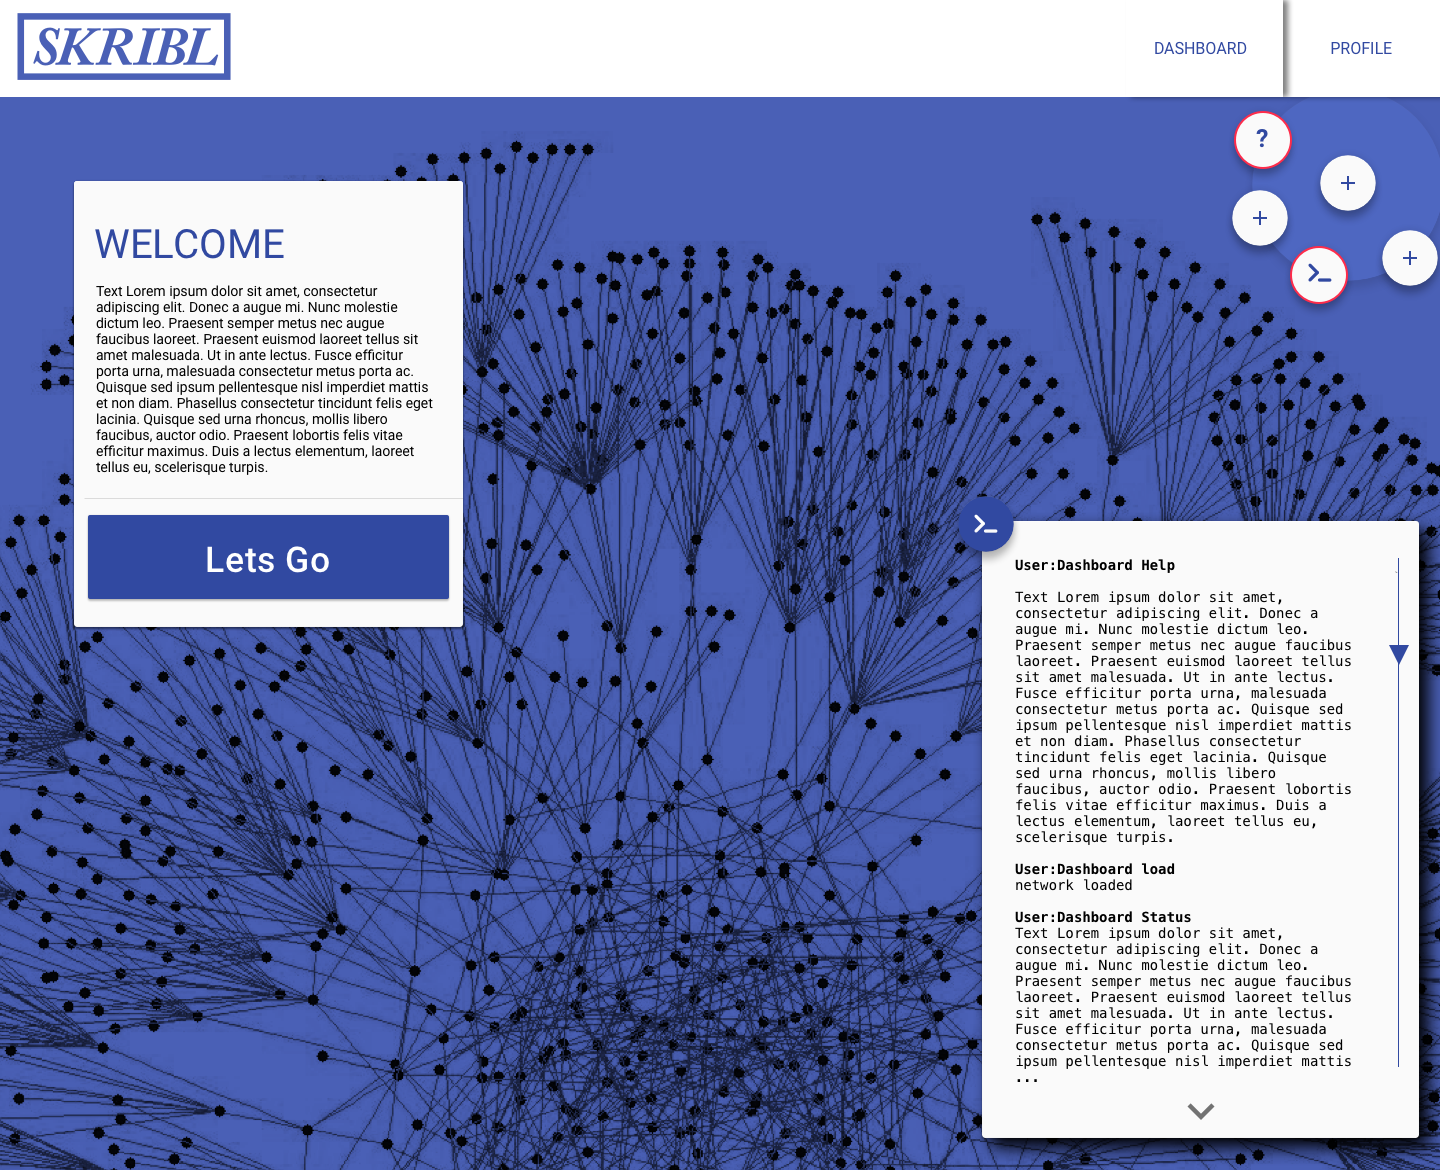
\includegraphics[width=140mm]{pieteruploads/SKRBL_FRNT_HomeGraph.png}
 \caption{Visualisatie de menus en CLI bij graph-view}
\end{figure}

\clearpage

\subsection{Datavisualisatie}
\begin{figure}[!h]
\centering
 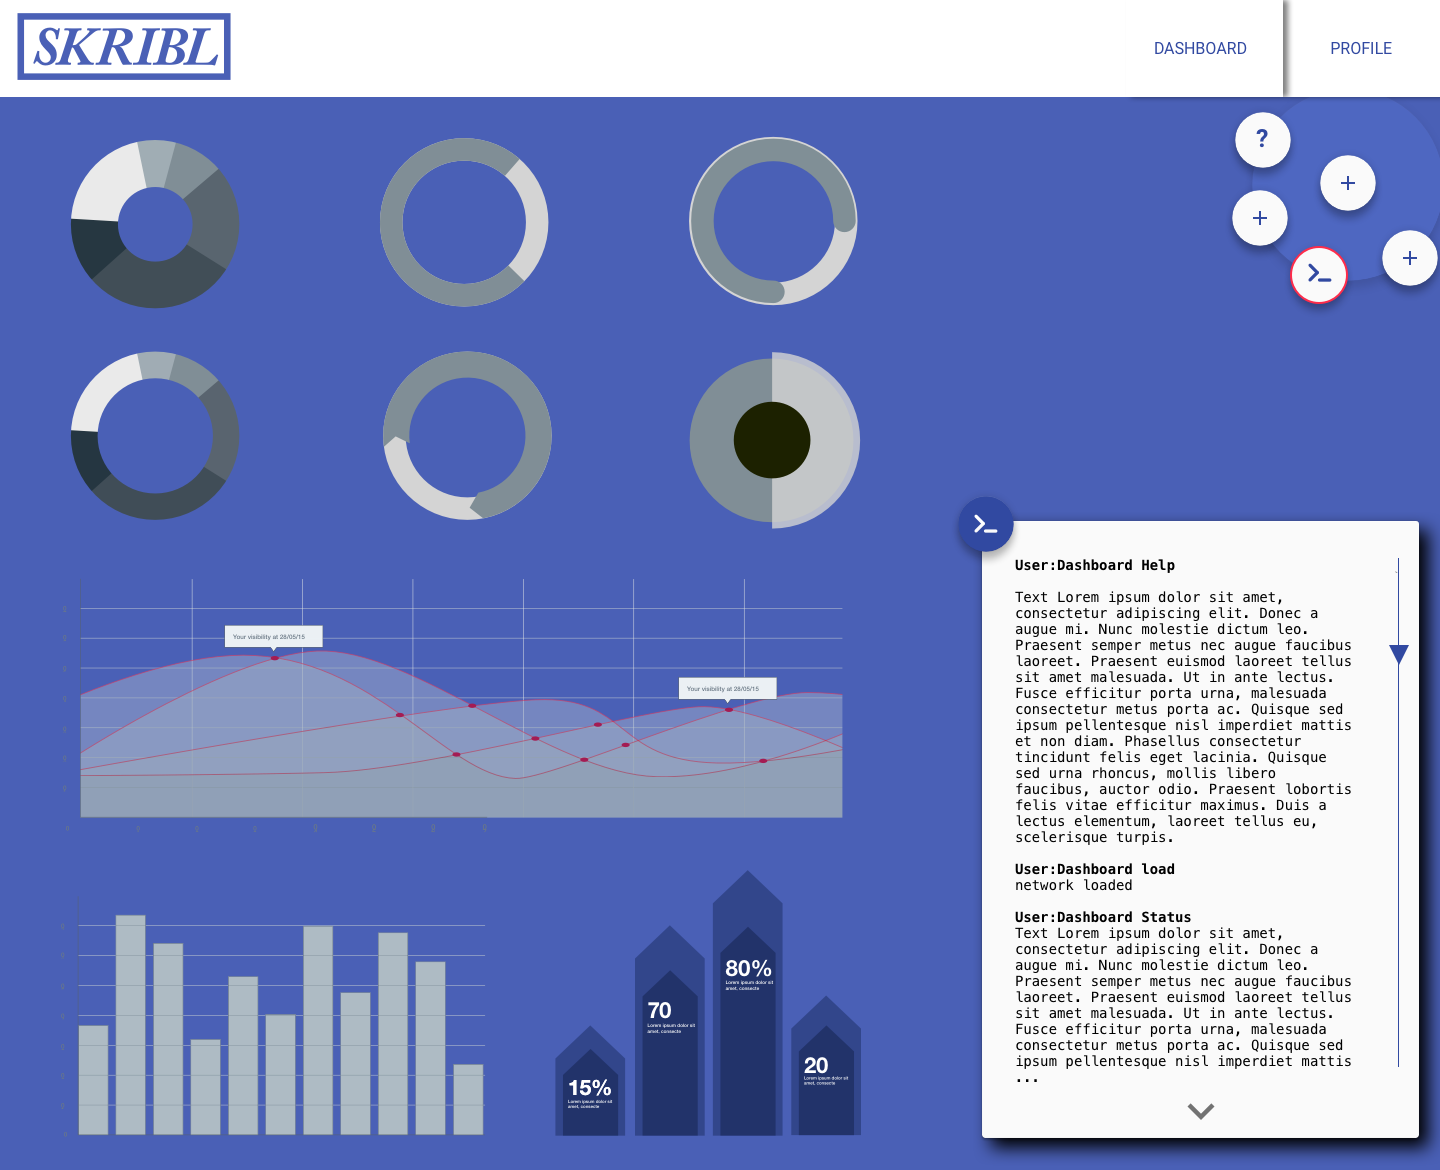
\includegraphics[width=140mm]{pieteruploads/SKRBL_FRNT_Dataviz.png}
 \caption{Visualisatie de menus en CLI bij een mock-up van de datavisualisatie}
\end{figure}

\clearpage
\end{appendices}

\end{document}
